\section{Referencia de la Clase Albaran\-Proveedor}
\label{classAlbaranProveedor}\index{AlbaranProveedor@{AlbaranProveedor}}
Clase que almacena los datos de un albar\'{a}n de proveedor.  


{\tt \#include $<$albaranproveedor.h$>$}

Diagrama de herencias de Albaran\-Proveedor\begin{figure}[H]
\begin{center}
\leavevmode
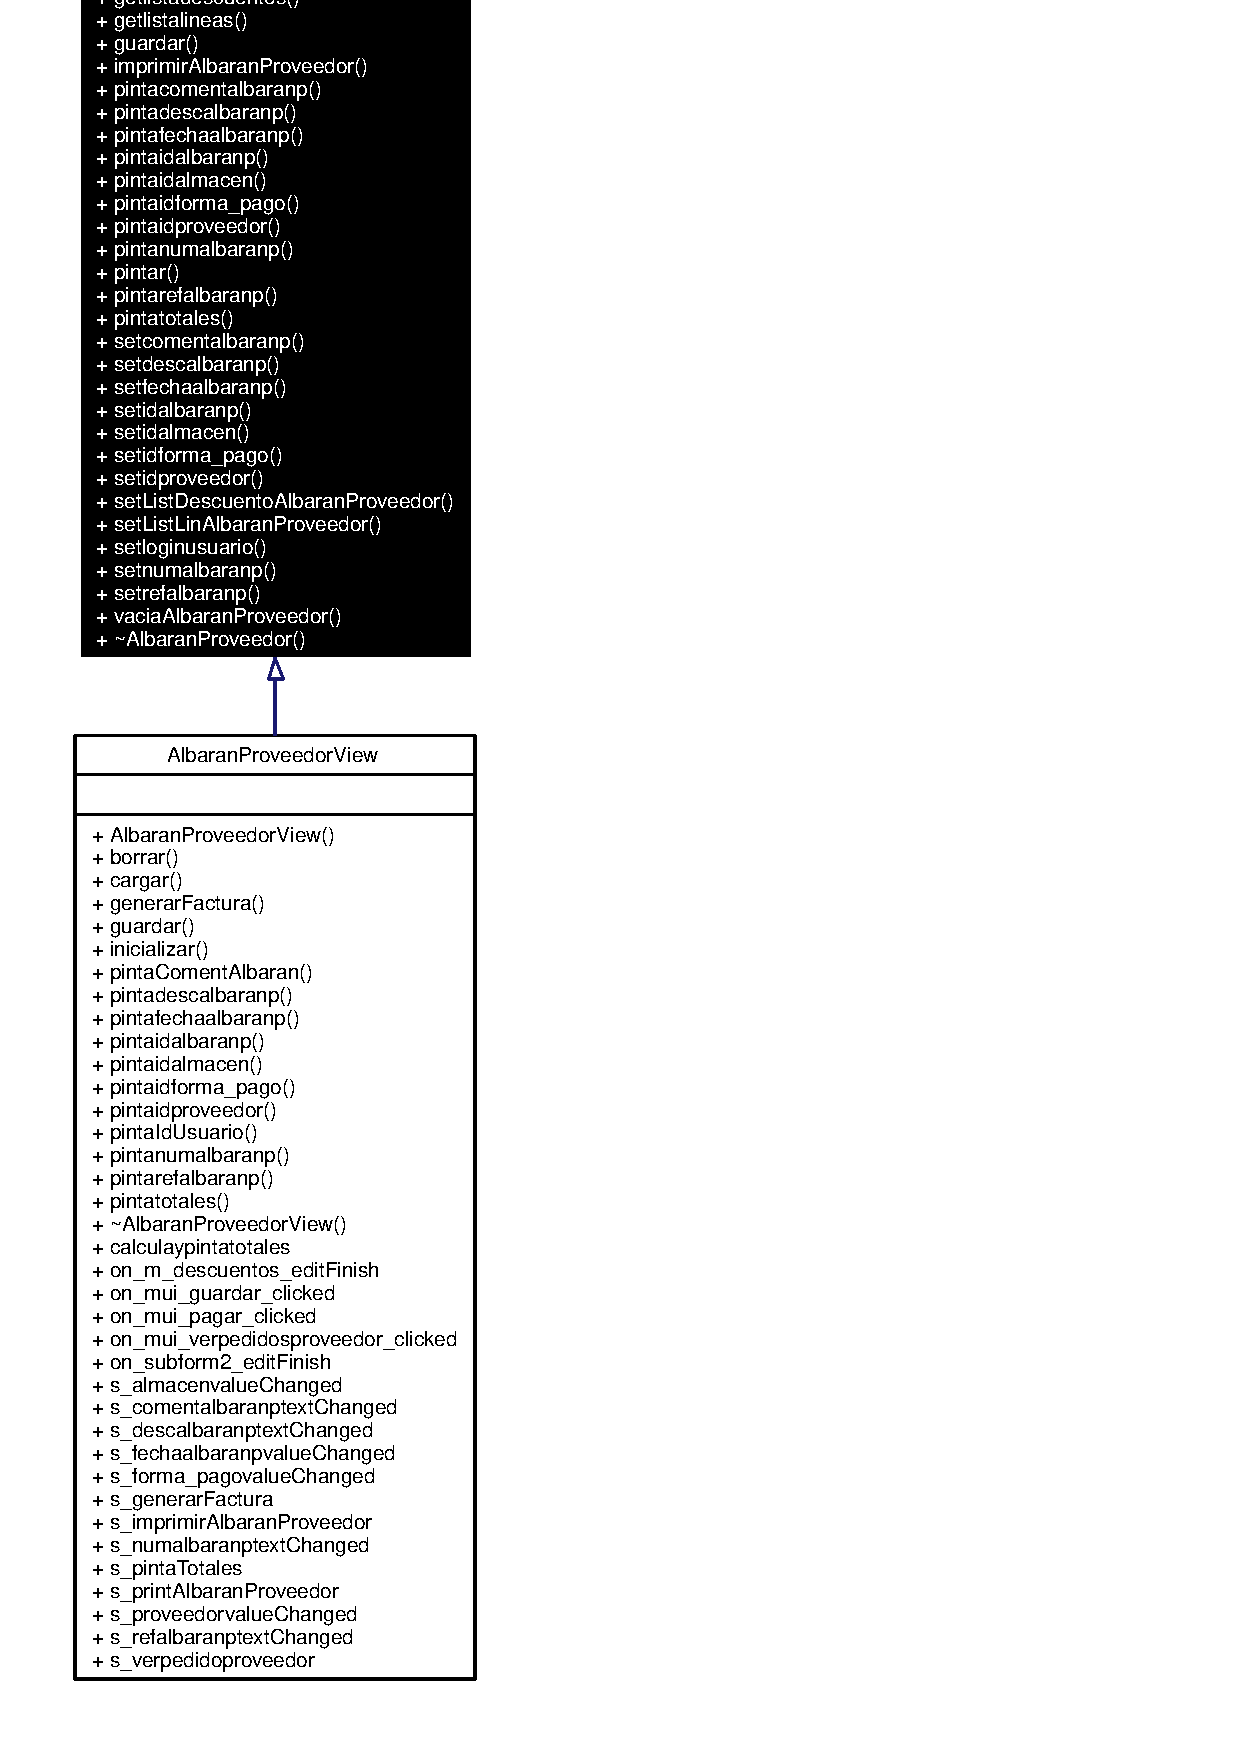
\includegraphics[width=114pt]{classAlbaranProveedor__inherit__graph}
\end{center}
\end{figure}
Diagrama de colaboraci\'{o}n para Albaran\-Proveedor:\begin{figure}[H]
\begin{center}
\leavevmode
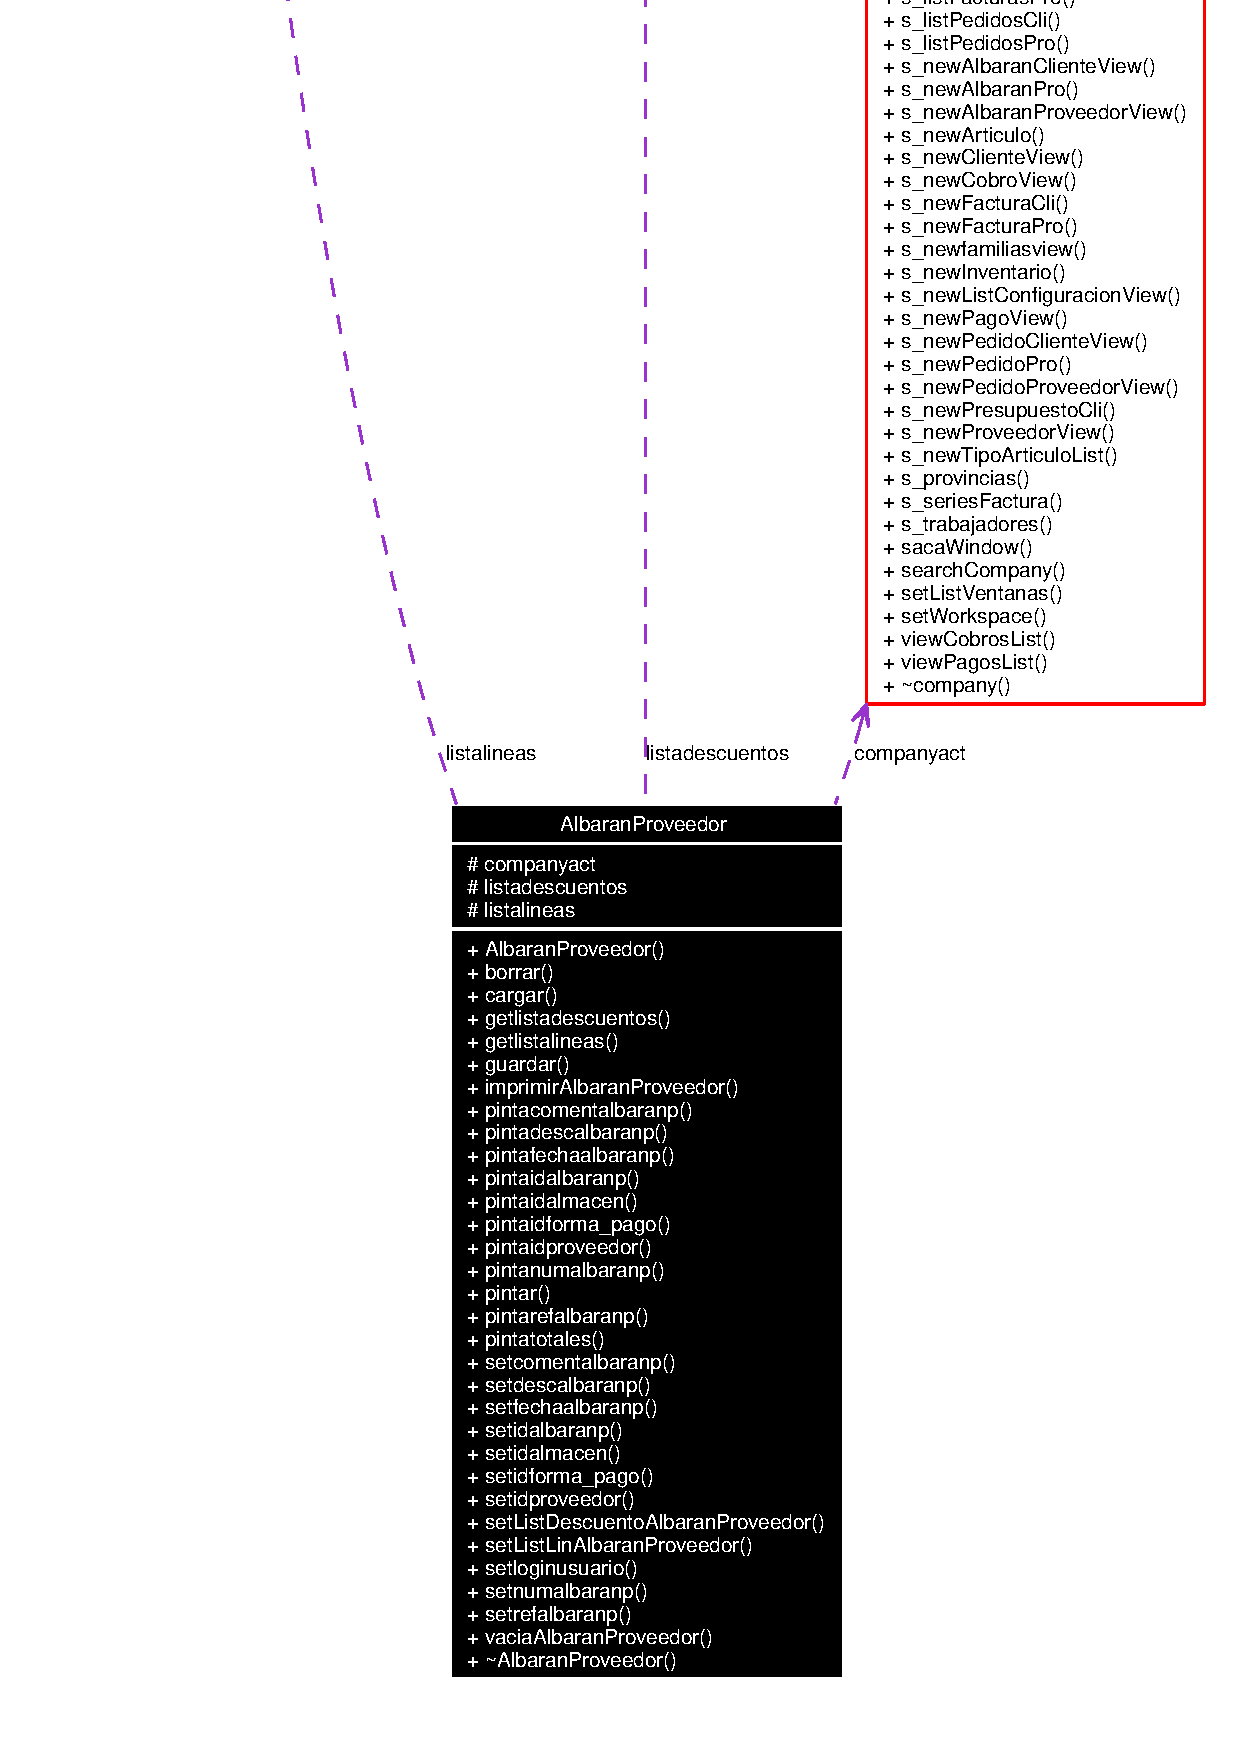
\includegraphics[width=289pt]{classAlbaranProveedor__coll__graph}
\end{center}
\end{figure}
\subsection*{M\'{e}todos p\'{u}blicos}
\begin{CompactItemize}
\item 
{\bf Albaran\-Proveedor} ({\bf company} $\ast$)\label{classAlbaranProveedor_a0}

\item 
virtual int {\bf borrar} ()\label{classAlbaranProveedor_a1}

\item 
virtual int {\bf cargar} (QString)\label{classAlbaranProveedor_a2}

\begin{CompactList}\small\item\em Esta funcion carga un Albaran\-Proveedor. \item\end{CompactList}\item 
{\bf List\-Descuento\-Albaran\-Prov\-View} $\ast$ {\bf getlistadescuentos} ()\label{classAlbaranProveedor_a3}

\item 
{\bf List\-Lin\-Albaran\-Proveedor\-View} $\ast$ {\bf getlistalineas} ()\label{classAlbaranProveedor_a4}

\item 
virtual int {\bf guardar} ()\label{classAlbaranProveedor_a5}

\item 
void {\bf imprimir\-Albaran\-Proveedor} ()
\item 
virtual void {\bf pintacomentalbaranp} (QString)\label{classAlbaranProveedor_a7}

\item 
virtual void {\bf pintadescalbaranp} (QString)\label{classAlbaranProveedor_a8}

\item 
virtual void {\bf pintafechaalbaranp} (QString)\label{classAlbaranProveedor_a9}

\item 
virtual void {\bf pintaidalbaranp} (QString)\label{classAlbaranProveedor_a10}

\item 
virtual void {\bf pintaidalmacen} (QString)\label{classAlbaranProveedor_a11}

\item 
virtual void {\bf pintaidforma\_\-pago} (QString)\label{classAlbaranProveedor_a12}

\item 
virtual void {\bf pintaidproveedor} (QString)\label{classAlbaranProveedor_a13}

\item 
virtual void {\bf pintanumalbaranp} (QString)\label{classAlbaranProveedor_a14}

\item 
virtual void {\bf pintar} ()
\item 
virtual void {\bf pintarefalbaranp} (QString)\label{classAlbaranProveedor_a16}

\item 
virtual void {\bf pintatotales} (Fixed, Fixed)\label{classAlbaranProveedor_a17}

\item 
void {\bf setcomentalbaranp} (QString val)\label{classAlbaranProveedor_a18}

\item 
void {\bf setdescalbaranp} (QString val)\label{classAlbaranProveedor_a19}

\item 
void {\bf setfechaalbaranp} (QString val)\label{classAlbaranProveedor_a20}

\item 
void {\bf setidalbaranp} (QString val)\label{classAlbaranProveedor_a21}

\item 
void {\bf setidalmacen} (QString val)\label{classAlbaranProveedor_a22}

\item 
void {\bf setidforma\_\-pago} (QString val)\label{classAlbaranProveedor_a23}

\item 
void {\bf setidproveedor} (QString val)\label{classAlbaranProveedor_a24}

\item 
void {\bf set\-List\-Descuento\-Albaran\-Proveedor} ({\bf List\-Descuento\-Albaran\-Prov\-View} $\ast$a)\label{classAlbaranProveedor_a25}

\item 
void {\bf set\-List\-Lin\-Albaran\-Proveedor} ({\bf List\-Lin\-Albaran\-Proveedor\-View} $\ast$a)
\item 
void {\bf setloginusuario} (QString val)\label{classAlbaranProveedor_a27}

\item 
void {\bf setnumalbaranp} (QString val)\label{classAlbaranProveedor_a28}

\item 
void {\bf setrefalbaranp} (QString val)\label{classAlbaranProveedor_a29}

\item 
void {\bf vacia\-Albaran\-Proveedor} ()\label{classAlbaranProveedor_a30}

\end{CompactItemize}
\subsection*{Atributos protegidos}
\begin{CompactItemize}
\item 
{\bf company} $\ast$ {\bf companyact}\label{classAlbaranProveedor_p0}

\item 
{\bf List\-Descuento\-Albaran\-Prov\-View} $\ast$ {\bf listadescuentos}\label{classAlbaranProveedor_p1}

\item 
{\bf List\-Lin\-Albaran\-Proveedor\-View} $\ast$ {\bf listalineas}\label{classAlbaranProveedor_p2}

\end{CompactItemize}


\subsection{Descripci\'{o}n detallada}
Clase que almacena los datos de un albar\'{a}n de proveedor. 



\subsection{Documentaci\'{o}n de las funciones miembro}
\index{AlbaranProveedor@{Albaran\-Proveedor}!imprimirAlbaranProveedor@{imprimirAlbaranProveedor}}
\index{imprimirAlbaranProveedor@{imprimirAlbaranProveedor}!AlbaranProveedor@{Albaran\-Proveedor}}
\subsubsection{\setlength{\rightskip}{0pt plus 5cm}void Albaran\-Proveedor::imprimir\-Albaran\-Proveedor ()}\label{classAlbaranProveedor_a6}


Copiamos el archivo.

Copiamos el logo.

Linea de totales del presupuesto. \index{AlbaranProveedor@{Albaran\-Proveedor}!pintar@{pintar}}
\index{pintar@{pintar}!AlbaranProveedor@{Albaran\-Proveedor}}
\subsubsection{\setlength{\rightskip}{0pt plus 5cm}void Albaran\-Proveedor::pintar ()\hspace{0.3cm}{\tt  [virtual]}}\label{classAlbaranProveedor_a15}


Pintamos los totales. \index{AlbaranProveedor@{Albaran\-Proveedor}!setListLinAlbaranProveedor@{setListLinAlbaranProveedor}}
\index{setListLinAlbaranProveedor@{setListLinAlbaranProveedor}!AlbaranProveedor@{Albaran\-Proveedor}}
\subsubsection{\setlength{\rightskip}{0pt plus 5cm}void Albaran\-Proveedor::set\-List\-Lin\-Albaran\-Proveedor ({\bf List\-Lin\-Albaran\-Proveedor\-View} $\ast$ {\em a})\hspace{0.3cm}{\tt  [inline]}}\label{classAlbaranProveedor_a26}


Establece cual es la lista subformulario del presupuesto. Normalmente para apuntar listlinpresupuestoview. 

La documentaci\'{o}n para esta clase fu\'{e} generada a partir de los siguientes archivos:\begin{CompactItemize}
\item 
albaranproveedor.h\item 
albaranproveedor.cpp\end{CompactItemize}
